\documentclass[10pt]{report}
\usepackage[utf8]{inputenc}
\usepackage{amsfonts}
\usepackage{amsmath}
\usepackage{amssymb}
\usepackage{commath}
\usepackage[ngerman]{babel}
\usepackage{enumitem}
\usepackage{booktabs}
\usepackage{longtable}
\usepackage{relsize}
\usepackage{pgfplots}
\usepackage{csvsimple}
\usepackage{pgfplotstable}
\usepackage{siunitx}
\usepackage{fancyhdr}

\setlength\parindent{0pt}

\setcounter{section}{-1} % TODO

\pagestyle{fancy}
\fancyhf{}
\lhead{GPET Versuch} % TODO
\rhead{Tim Luchterhand, Paul Nykiel}
\cfoot{\thepage}

\begin{document}
        \section{Messwerte mit Python}
        Leider wurde das Multimeter am Computer nicht erkannt.

        \begin{table}[h!]
            \begin{center}
                \caption{Messwerte für Stromfehlerschaltung}
                \label{table1}
                \pgfplotstabletypeset[
                multicolumn names, % allows to have multicolumn names
                col sep=space, % the seperator in our .csv file
                display columns/0/.style={
                column name=$U_B$, % name of first column
                column type={S},string type},  % use siunitx for formatting
                display columns/1/.style={
                column name=$U_x$,
                column type={S},string type},
                display columns/2/.style={
                column name=$I$,
                column type={S},string type},
                display columns/3/.style={
                column name=$R_x$,
                column type={S},string type},
                display columns/4/.style={
                column name=$\Delta R$,
                column type={S},string type},
                display columns/5/.style={
                column name=$\rho_R$,
                column type={S},string type},
                every head row/.style={
                before row={\toprule}, % have a rule at top
                after row={
                \si{\volt} & \si{\volt} & $\mu$\si{\ampere} & k\si{\ohm} & k\si{\ohm} & \%\\
                \midrule} % rule under units
                },
                every last row/.style={after row=\bottomrule},
                ]{widerstandskennlinie.csv}
            \end{center}
        \end{table}

        \subsection{U-I-Diagram}
        \begin{center}
            \begin{tikzpicture}
        		\begin{axis}[ymin=0, xlabel = {V}, ylabel = {$\mu$ A}]
        			\addplot table[x index = {1},
                            y index = {2}] {widerstandskennlinie.csv};
        		\end{axis}
        	\end{tikzpicture}
        \end{center}

        \noindent Das Diagram zeigt eine Gerade mit Steigung R. Die Kurve hätte ein Offset am
        Schnittpunkt mit der y-Achse, dieser ist der Messungenauigkeit bei 5V
        geschuldet.

        \section{Oszilloskop}
        Nach Betrachtung der Skalierung erkennt man das eine Periode genau 5 Blöcke
        mit jeweils $2 \mu$s dauert, die Frequenz ist also 1kHz, wie eingestellt.
        \begin{figure}
         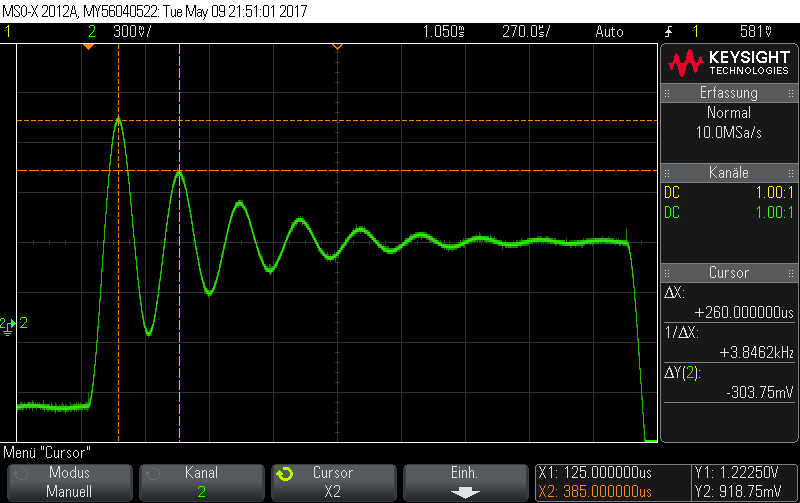
\includegraphics[width=\textwidth]{scope_13.png}
         \caption{Frequenzmessung}
       \end{figure}

       \subsection{Trigger}

        Der Anfang der Messung ist an dem Punkt an dem der Trigger zum ersten mal
        ausgelöst wird. Somit verschiebt sich das Bild wenn man das Trigger Level
        ändert.

         \noindent Sobald das Trigger Level höher bzw.\ niedriger als das Signal sind wird
         der Trigger nicht ausgelöst, es wird also nicht gemessen. Es wird kein sinnvolles
         Signal angezeigt.

         \section{DC-AC Einstellung}
         \textbf{DC:}\@ Das Signal ist um das eingestellte Offset verschoben.
         \begin{figure}
          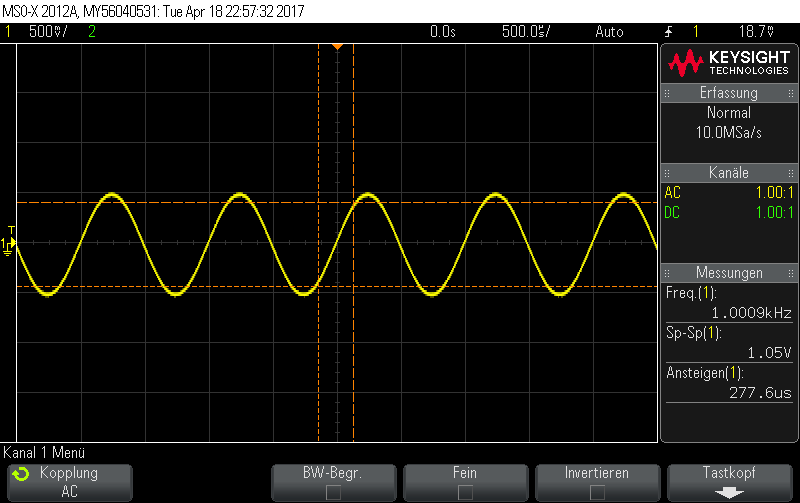
\includegraphics[width=\textwidth]{scope_5.png}
          \caption{DC}
        \end{figure}

         \noindent \textbf{AC:}\@ Das Signal wird ohne Verschiebung angezeigt, da Gleihanteile heraus
         gefiltert werden.
         \begin{figure}
          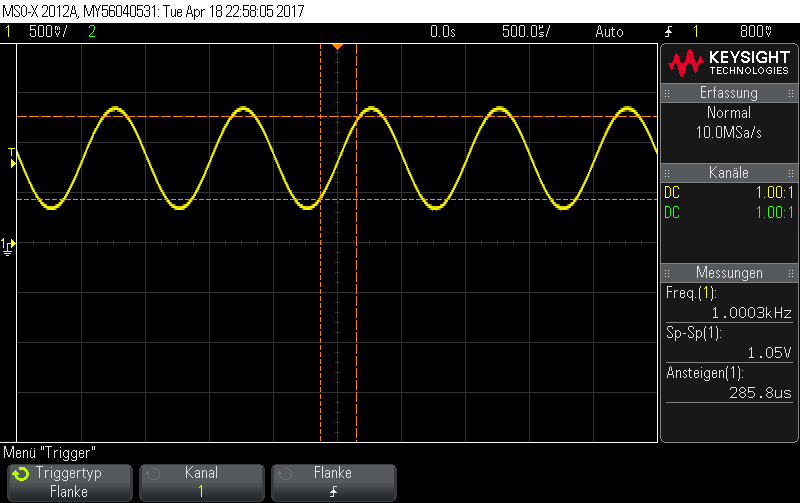
\includegraphics[width=\textwidth]{scope_6.png}
          \caption{AC}
        \end{figure}

         \noindent \textbf{Signalverzerrung:} Das verwendete Rechtecksignal hat eine Amplitude von 1 Volt pp
         und eine Frequenz von 100 Hz.
         \begin{figure}
          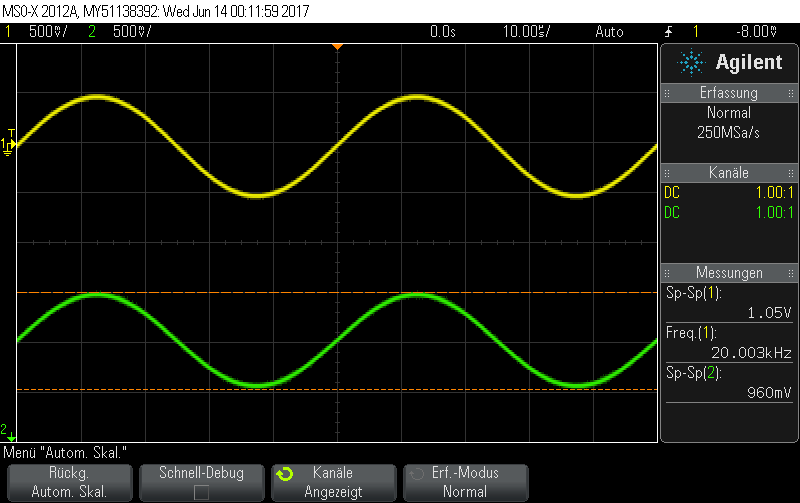
\includegraphics[width=\textwidth]{scope_1.png}
          \caption{Signalverzerrung}
        \end{figure}

         \noindent \textbf{Beobachtung:} Die horizontalen Kanten des Rechtecksignals sind nicht parallel
         zur x-Achse sondern werden in jedem Duty-cycle betragsmäßig mit der Zeit kleiner.

         \section{Kondensatormessung}
         \begin{figure}
          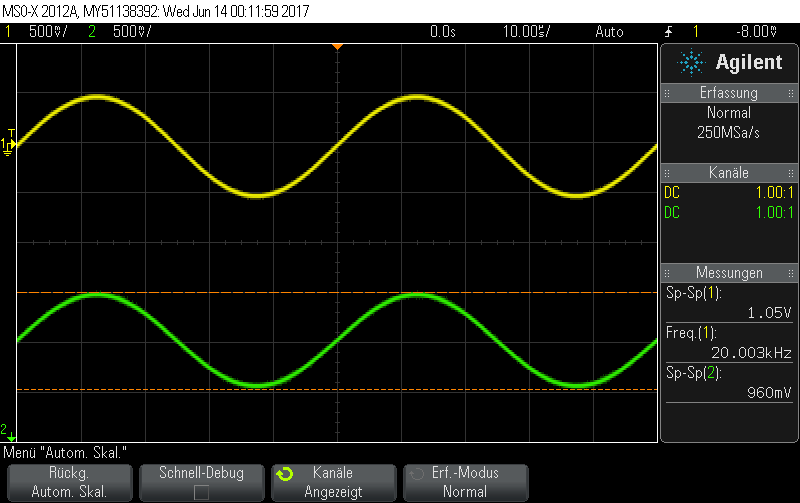
\includegraphics[width=\textwidth]{scope_1.png}
          \caption{Signal}
        \end{figure}
        \subsection{Messergebnisse mit Cursor}
        \begin{eqnarray*}
            \Delta x = 24 \mu s &\Rightarrow& \tau =  11 \mu s \\
            \tau = RC &\Rightarrow& C = \frac{\tau}{R}\\
            &\Rightarrow& C=218\text{nF}
        \end{eqnarray*}
        \begin{figure}
         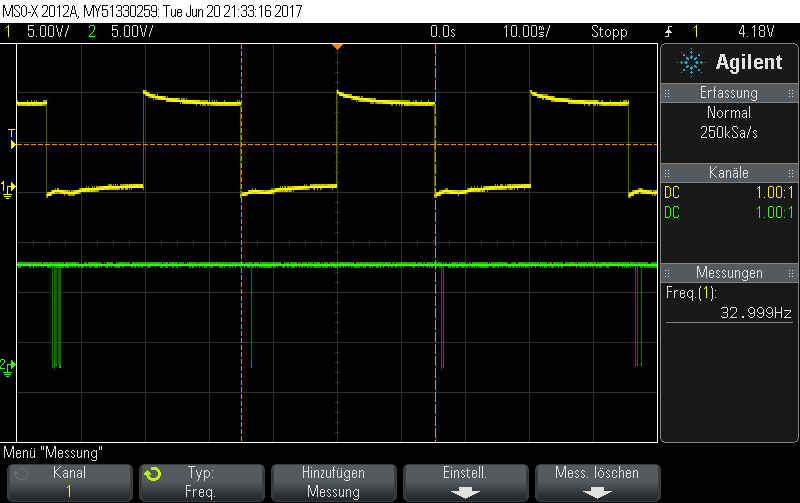
\includegraphics[width=\textwidth]{scope_2.png}
         \caption{Messung mit Cursor}
       \end{figure}

       \subsection{Messergebnisse mit Measure}
       \begin{eqnarray*}
           \Delta x = 9,74 \mu s &\Rightarrow& \tau =  4,43 \mu s \\
           \tau = RC &\Rightarrow& C = \frac{\tau}{R}\\
           &\Rightarrow& C=88.5\text{nF}
       \end{eqnarray*}
       \begin{figure}
        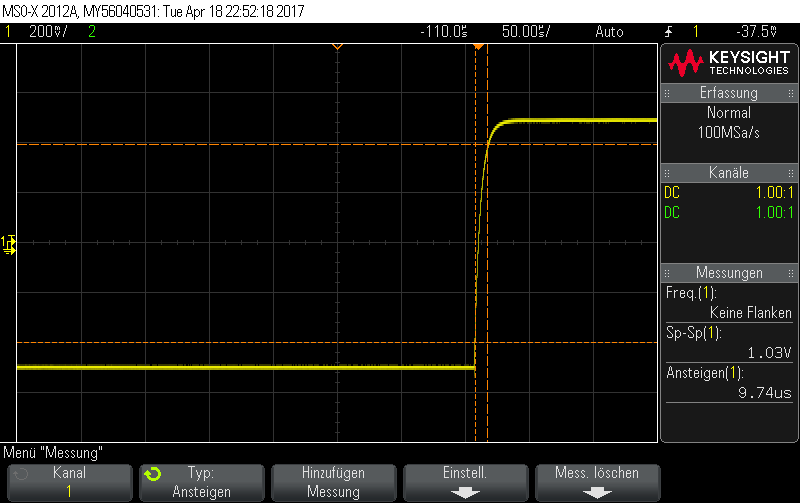
\includegraphics[width=\textwidth]{scope_4.png}
        \caption{Messung mit Measure}
      \end{figure}

      \subsection{Messergebnisse mit Multimeter}
      \begin{equation*}
          C = 97\text{nF}
      \end{equation*}

      \subsection{Abweichung}
      Vor allem zwischen der Messung mit Cursor und den beiden anderen Messungen
      ist ein großer Unterschied zu vermerken. Das liegt vor allem daran, dass die
      Anstiegszeiten manuell bestimmt werden mussten und dementsprechend ungenau sind.


      \section{Tiefpass}
      Grenzfrequenz: $1.9$kHz

      \noindent Phasenverschiebung bei Grenzfrequenz: $49^\circ$
      \begin{figure}
       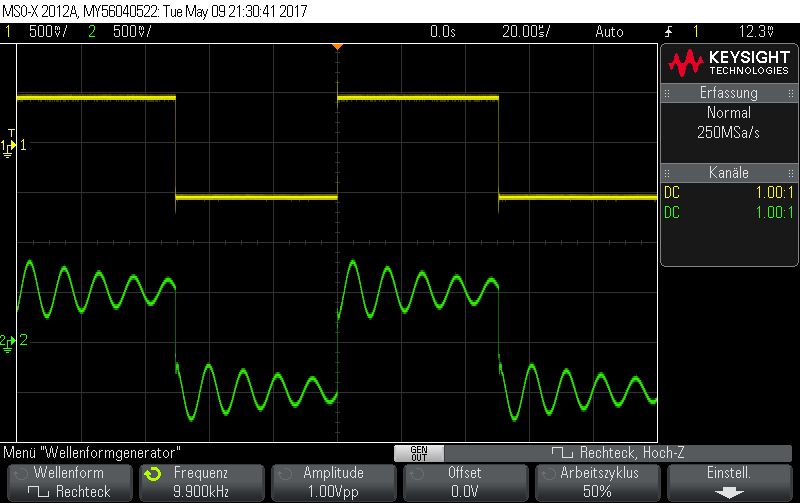
\includegraphics[width=\textwidth]{scope_8.png}
       \caption{Grenzfrequenz mit Cursor}
     \end{figure}

     \begin{figure}
      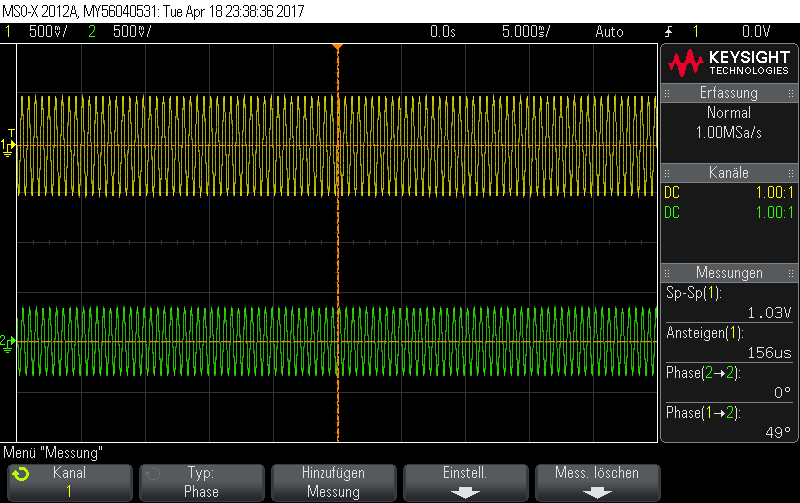
\includegraphics[width=\textwidth]{scope_9.png}
      \caption{Phasenverschiebung bei Grenzfrequenz}
    \end{figure}

    \section{Tastkopf}
    \begin{figure}
     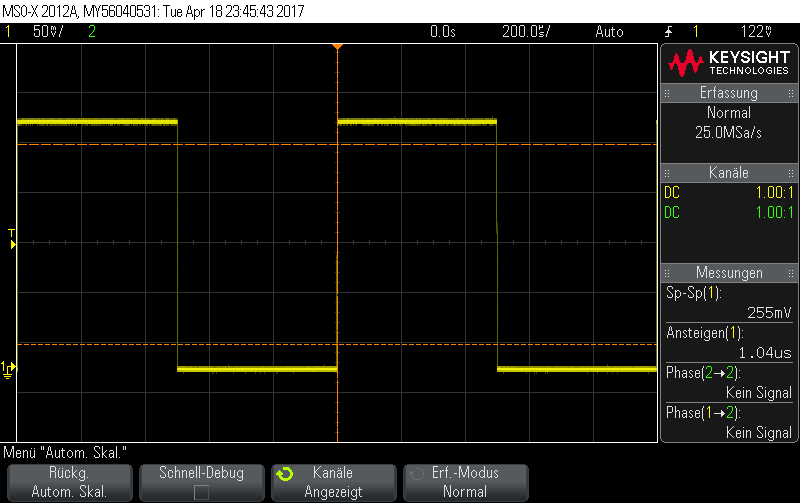
\includegraphics[width=\textwidth]{scope_12.png}
     \caption{Optimale Rechteckform}
   \end{figure}

   \begin{figure}
    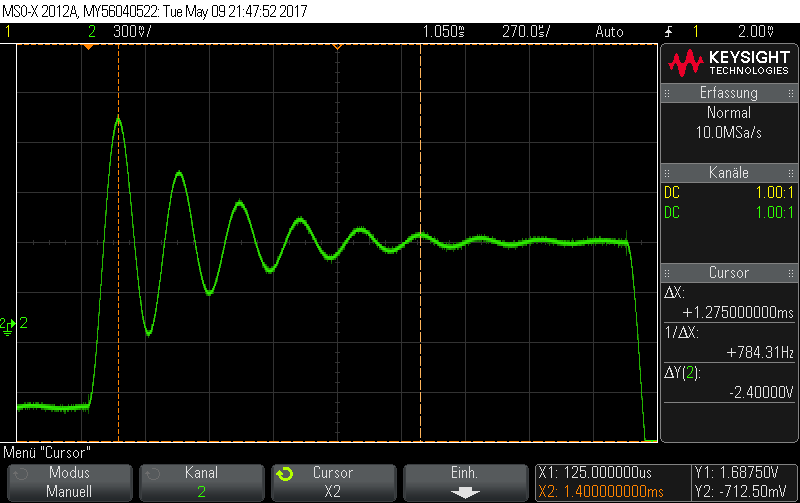
\includegraphics[width=\textwidth]{scope_11.png}
    \caption{Überschwingen}
  \end{figure}

  \begin{figure}
   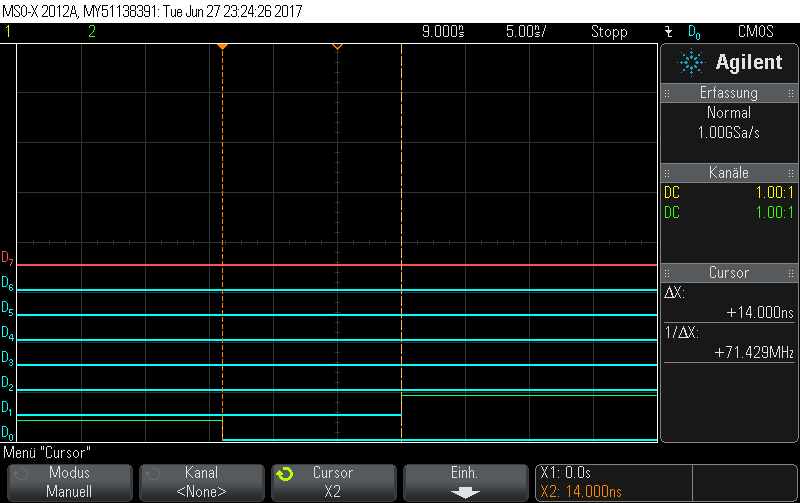
\includegraphics[width=\textwidth]{scope_10.png}
   \caption{Unterschwingen}
 \end{figure}


\end{document}
